%-------------------------------------------------------------
% Language
% Use the option "language=EN" to set the beamer theme in English. Use
% the option "language=ES" to set the beamer theme in Spanish.

% Colors
% Use the option "color=white" to set the background in white and the
% bottom bar in blue. Use the option "color=blue" to set the
% background in blue and the bottom bar in white. Use the option
% "color=blue2" to set the background in blue and the bottom bar in
% blue.

% Font Color
% Use the option "fontc=black" to set the font color in black. If this
% argument is not given the default color is set depending of the
% color scheme selected.

% Credits: https://github.com/alejogm0520 & Samuel Plazas Escudero
%-------------------------------------------------------------

%--Principal packages
\documentclass[xcolor=table, aspectratio=43,8pt]{beamer} % 4:3; can be 16:9; [...,8pt,t] in order to start text of all frames on the upper part; add: draft to not compile figures.
\usetheme[language=ES, color=white]{EAFIT}
\usepackage[spanish]{babel}
\decimalpoint % All decimal numbers with point
\usepackage[utf8]{inputenc}

\selectlanguage{spanish}
\usepackage{amsmath,amsfonts,amssymb,cancel} % Equations; physics is optional and sometimes problematic!
\usepackage{verbatim} % Environments, \begin{comment}
%--Arial
\usepackage{helvet}\renewcommand{\familydefault}{\sfdefault}% It's ok


\newcommand{\ihat}{\hat{\mathbf{i}}}
\newcommand{\jhat}{\hat{\mathbf{i}}}
\newcommand{\khat}{\hat{\mathit{k}}}
%--David Plazas recommended
%\usepackage{libertine} % Normal
%--Carlos Cuartas
%\usepackage[T1]{fontenc}\usepackage{lmodern} % Best
%--Beamer packages
\usepackage{tikz} % For making vectorized figures, arrows
\usepackage{ifthen} % For specifying conditionals for sections
\usepackage{ragged2e}\justifying % Whole text justified, except enumerate: add \justifying
\usepackage{multicol} % Multiple columns in one frame
%--Tables-Figures
\renewcommand\spanishtablename{Tabla}
\usepackage{booktabs,multirow} % Bookstyle tables
\usepackage{array} % Custom width and centered
\newcolumntype{P}[1]{>{\centering\arraybackslash}p{#1}} % horizotnal centering but use custom width
\newcolumntype{M}[1]{>{\centering\arraybackslash}m{#1}} % horizotnal and vertical centering but use custom width
%-Figure label
\usepackage[labelsep=period,justification=justified,format=plain]{caption} % Dot instead of colon and justified caption
%--Figure
\usepackage{graphicx,subcaption} % Figures and subfigures
\graphicspath{{Media/}} % Media rute
\usepackage{media9} % video and audio
%-Figure-Table on top
\usepackage{float} % Allows to put H instead of ht
\setbeamertemplate{caption}[numbered] % Numbered captions
%---------TOC
\setbeamertemplate{section in toc}[sections numbered]
\setbeamertemplate{subsection in toc}[subsections numbered]
\setbeamerfont{section in toc}{size=\small}
\setbeamerfont{subsection in toc}{size=\footnotesize}
\setbeamertemplate{subsection in toc}{\leavevmode\leftskip=3.2em\rlap{\hskip-2em\inserttocsectionnumber.\inserttocsubsectionnumber}\inserttocsubsection\par} % Indented subsection
\setcounter{tocdepth}{2} % Toc depth, put 1 for only showing there the sections and 2 to include sections
%---------Cite
\usepackage{bibentry} % Full cite foot
\nobibliography* % Full cite foot
\setbeamertemplate{bibliography item}[triangle]% [online][book][article][triangle][text]; Or: \setbeamertemplate{bibliography item}{\insertbiblabel}
\usepackage{etoolbox} % Package for using justified bibliography
\apptocmd{\thebibliography}{\justifying}{}{} % Justified bibliography
%---------Footnotes
\setbeamercolor{footnote}{fg=white} % Footnote white
\setbeamercolor{footnote mark}{fg=.} % Takes the color depending on the circumpstance
\setbeamercolor{bibliography entry author}{fg=white} % Allows to have white footnote bibs
\setbeamertemplate{footnote}
{
  \hspace*{-1cm} % Horizontal movement
  \vspace*{-3.2cm} % Vertical movement
  \parbox[c][3.64cm]{10.6cm}{\tiny\noindent\insertfootnotemark\insertfootnotetext} % b: bottom, height: 3.3cm, horizontal length: 10.6cm (max horizontal) standar = 3.12
% If there are problems, put \vspace*{-2.87cm} and \parbox[c][3.3cm]
% or \vspace*{-2.88cm} and \parbox[c][3.4cm]
% or \vspace*{-3.05cm} and \parbox[c][3.6cm]
% or \vspace*{-3.12cm} and \parbox[c][3.64cm]
}
\renewcommand{\footnoterule}{\kern -3pt \hrule width \textwidth height 0pt\kern 3pt} % No footnoterule
\usepackage{perpage}\MakePerPage{footnote} % Footnote numbered per frame
\renewcommand{\thefootnote}{\Roman{footnote}} % Roman number in footnote
                                              % Cutom: \fnsymbol{footnote}
%------------------------------------
%---------Numbered Slides and Sections
\setbox0=\hbox{\subsecname\unskip}\ifdim\wd0=0pt\else%
 ~--~\insertsubsectionhead
\fi
%------Numbering section: title in bold, centered and with a line
\newcommand{\numb}
{
  \setbeamertemplate{frametitle}
  {
    \ifx\insertsubsection\empty % No subsection
         \bfseries\thesection.~\insertframetitle~\color{black}\par\vskip-5pt\hrulefill % \centering
    \else % subsection
         \bfseries\thesection.~\insertframetitle~\color{black}\par\vskip-9pt\hrulefill\par\vskip3pt{\large\thesection.\thesubsection~\insertframesubtitle} % Subsection with smaller size;
    \fi
  }
}
%------No numbering section: title in bold, centered and with a line
\newcommand{\nonumb}
{
  \setbeamertemplate{frametitle}{\bfseries\color{black}\centering\insertframetitle\par\vskip-6pt\hrulefill}
}
%------------------------------------
%--No hyphenation on text
\tolerance=1
\emergencystretch=\maxdimen
\hyphenpenalty=10000
\hbadness=10000
%------------------------
%---------Itemize justified in beamer
\makeatletter
\renewcommand{\itemize}[1][]{
  \beamer@ifempty{#1}{}{\def\beamer@defaultospec{#1}}
  \ifnum \@itemdepth >2\relax\@toodeep\else
    \advance\@itemdepth\@ne
    \beamer@computepref\@itemdepth % Sets \beameritemnestingprefix
    \usebeamerfont{itemize/enumerate \beameritemnestingprefix body}
    \usebeamercolor[fg]{itemize/enumerate \beameritemnestingprefix body}
    \usebeamertemplate{itemize/enumerate \beameritemnestingprefix body begin}
    \list
      {\usebeamertemplate{itemize \beameritemnestingprefix item}}
      {\def\makelabel##1{
          {
            \hss\llap{{
                \usebeamerfont*{itemize \beameritemnestingprefix item}
                \usebeamercolor[fg]{itemize \beameritemnestingprefix item}##1}}
          }
        }
      }
  \fi
  \beamer@cramped
  \justifying % Justified itemize
  \beamer@firstlineitemizeunskip
}
\makeatother
%------------------------
%---------get current section name for showing it at its begining
\usepackage{nameref}
\makeatletter
\newcommand*{\currentname}{\@currentlabelname}
\makeatother
%---------Shows in which section we are at the begining of each one
%\begin{comment}
\AtBeginSection[]
{
\begin{frame}[plain,noframenumbering]
  \begin{beamercolorbox}[ht=\paperheight,wd=\paperwidth, center]{Portada}
    \begin{center}\textbf{\LARGE \currentname}\end{center} % Leave the next space mandatorily

    \vspace{0.44\paperheight}
  \end{beamercolorbox}
\end{frame}
}
%\end{comment}

%-------------------(CONSTANTLY BEING EDITED)------------------
%---------TEXTBLOCKS-GRID
\usepackage[absolute,overlay,showboxes]{textpos}
%\usepackage[texcoord,grid,gridunit=mm,gridcolor=red!10,subgridcolor=green!10]{eso-pic} % Helping grids, comment when publishing
%---------NOTES IN BEAMER
\AtBeginNote{\Huge}\newcommand{\notei}[1]{\note[item]{\Huge{\textcolor{blue}{#1}}}} % Use \notei{text} everywhere % [1] means one parameter located in #1 (input).
\setbeamertemplate{note page}[plain] % Plain style for notes page
\setbeameroption{show notes} % {show notes} or {hide notes}
% \setbeameroption{show notes on second screen=right}
% as well you can use \documentclass[notes=only] at the beginning of the code
%-----------More elaborated notes
%\setbeamercolor{note page}{bg=white!90!black, fg=black}
%\setbeamercolor{note title}{bg=white!30!red, fg=black}
%\setbeamercolor{note date}{parent=note title}
%---------Itemize, enumberate and lists inside them
%\setbeamertemplate{itemize/enumerate body begin}{\LARGE} % Body
\setbeamertemplate{itemize/enumerate subbody begin}{\Large} % Subbody
%---------COLOR DEFINITIONS
\definecolor{azure(colorwheel)}{rgb}{0.0, 0.5, 1.0} % Define colors here
\definecolor{blue(ryb)}{rgb}{0.01, 0.28, 1.0}

\usepackage{subcaption}


%%%%%%%%%%%%%%%%%%%%%%%
%Start of the Document%
%%%%%%%%%%%%%%%%%%%%%%%

%---------COVER PAGE
\title{FENÓMENOS ONDULATORIOS}
\author{\normalfont\texorpdfstring{Presentado por:\\Mariana Escobar Q.\\Juan S. Cárdenas R. \\ David Plazas E.\\[1ex] Profesor: MSc. Alejandro Madrid S.}{}}


\def\departamento{Departamento de Ciencias Físicas}
\def\escuela{Escuela de Ciencias}
\def\eafit{Universidad EAFIT}
\def\materia{Física II}
\def\fecha{2018} % or put the exact date
% to add more def, search for "Dirección" in beamerthemeEAFIT.sty
%\includeonly{Slides/0_cover_title,ex_beamer,Slides/refs_thanks}
\begin{document}


\nonumb % Not numbered titles
\begin{frame}
% Portada Inspira Crea Transforma
\end{frame}
%%%%%%%%%%%%%%%%%%%%%%%%%%%%%%%%%%%%%%%%%%%%%%%%%%%%%%%%%%%%%%%%%%%%%%%%%%%%
\begin{frame}
\begin{center}
  \titlepage % Cover page
\end{center}
\end{frame}
%%%%%%%%%%%%%%%%%%%%%%%%%%%%%%%%%%%%%%%%%%%%%%%%%%%%%%%%%%%%%%%%%%%%%%%%%%%%
\begin{frame}{CONTENIDO}
\begin{multicols}{2}
  \tableofcontents
\end{multicols}
\end{frame}
\numb % Numbered titles
%%%%%%%%%%%%%%%%%%%%%%%%%%%%%%%%%%%%%%%%%%%%%%%%%%%%%%
\section{OBJETIVOS}
%%%%%%%%%%%%%%%%%%%%%%%%%%%%%%%%%%%%%%%%%%%%%%%%%%%%%%%%%
\begin{frame}{OBJETIVOS}
    \Large{\begin{itemize}
        \item Introducir a los diferentes fenómenos e interacciones de las ondas electromagnéticas a través de teoría y experimentos.
        \item Dar una idea acerca de las aplicaciones actuales de los fenómenos e interacciones de las ondas electromagnéticas.
    \end{itemize}}
\end{frame}


\section{CONCEPTOS}
\subsection{}

\begin{frame}{CONCEPTOS}
  \begin{itemize}
    \item \textbf{Onda electromagnética}: Son ondas que no necesitan un medio para propagarse. Están compuestas de un campo magnético y uno eléctrico, ortogonales entre sí.
    \item \textbf{Longitud de onda (\boldmath$\lambda$)}: Distancia recorrida en un periodo.
    \item \textbf{Frente de onda:} Planos en los que el campo magnético y eléctrico son constantes.
    \item \textbf{Luz visible}: Intervalo del espectro electromagnético de $\lambda$ entre 400nm y 750 nm. Para el caso de reflexión y refracción se considera como un haz, pero también funciona para el modelo ondulatorio.
    \item \textbf{Ángulo de incidencia}: Ángulo con el que llega la onda al objeto de estudio. Se mide desde la normal a éste.
    \item \textbf{Imagen virtual:} Es la imagen formada cuando los rayos salientes divergen.
  \end{itemize}
\end{frame}
%%%%%%%%%%%%%%%%%%%%%%%%%%%%%%%%%%%%%%%%%%%%%%%%%%%%%%%%%%

\section{REFRACCIÓN}
\subsection{Concepto}

\begin{frame}{REFRACCIÓN}
  \framesubtitle{Concepto}
  \begin{itemize}
    \item Cuando una onda electromagnética pasa de una medio a otro, se desvía respecto al ángulo incidente.
    \item Puede ocurrir al mismo tiempo que la reflexión\footnote{\bibentry{sears}}.
  \end{itemize}
  \begin{figure}
      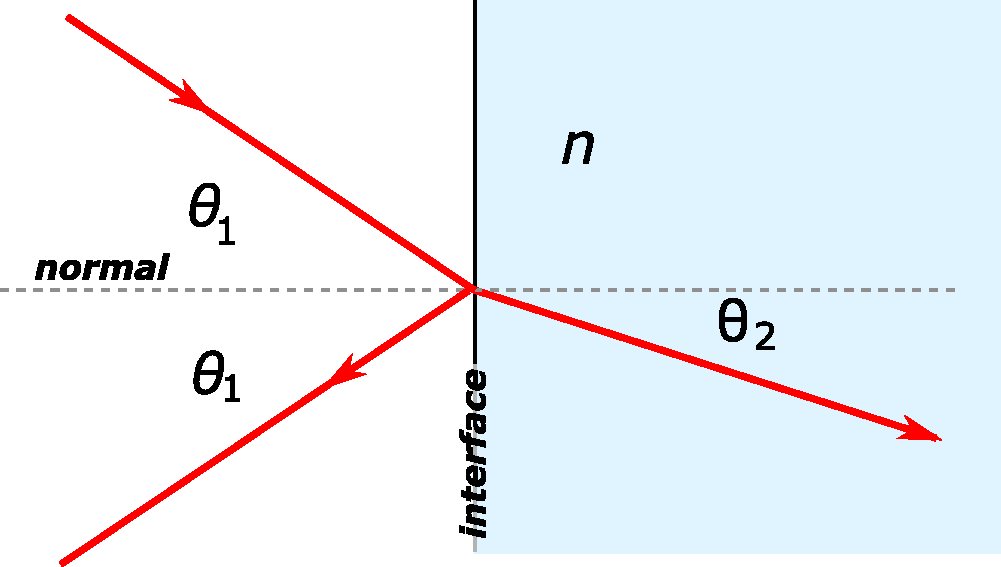
\includegraphics[scale=0.4]{david/Refrac.pdf}
      \caption{Reflexión y refracción\footnotemark{}.}
  \end{figure}
  \vspace{-2cm}\footnotetext{\bibentry{refrac}}
\end{frame}

\subsection{Índice de Refracción}

\begin{frame}{REFRACCIÓN}
  \framesubtitle{Índice de Refracción}
  Razón entre la rapidez de la luz en el vacío $c$ y la rapidez en un material $v$.
  \begin{equation}
    n = \frac{c}{v}
  \end{equation}
  La luz siempre viaja \textit{más lento} en un material que en el vacío\footnote{\bibentry{sears}}.

  \begin{table}[H]
    \centering
    \caption{Índices de refracción para diferentes materiales.}
    \begin{tabular}{cc}
    \hline
    \textbf{Material} & \textbf{Índice de Refracción (n)} \\ \hline
    Vacío             & 1                                 \\
    Aire              & 1,0002926                         \\
    Etanol            & 1,361                             \\
    Agua              & 1,3330                            \\
    Diamante          & 2,419                             \\
    Ámbar             & 1,55                              \\
    Hielo             & 1,31                              \\
    Córnea humana     & 1,3375                            \\ \hline
    \end{tabular}
\end{table}

\end{frame}

\subsection{Ley de Snell}
\begin{frame}{REFRACCIÓN}
    \framesubtitle{Ley de Snell}
    \begin{enumerate}
        \item Rayo incidente, reflejado, refractado y la normal están todos en un mismo plano. Plano ortogonal a la superficie que limita los medios.
        \item Razón entre los $\sin$ de los ángulos incidente y refractado es igual al inverso de los índices de refracción:
    \end{enumerate}
    \begin{equation}
        \frac{\sin \theta_a}{\sin \theta_b}=\frac{n_b}{n_a}\longrightarrow n_b\sin\theta_b=n_a\sin\theta_a
    \end{equation}
    \begin{figure}
        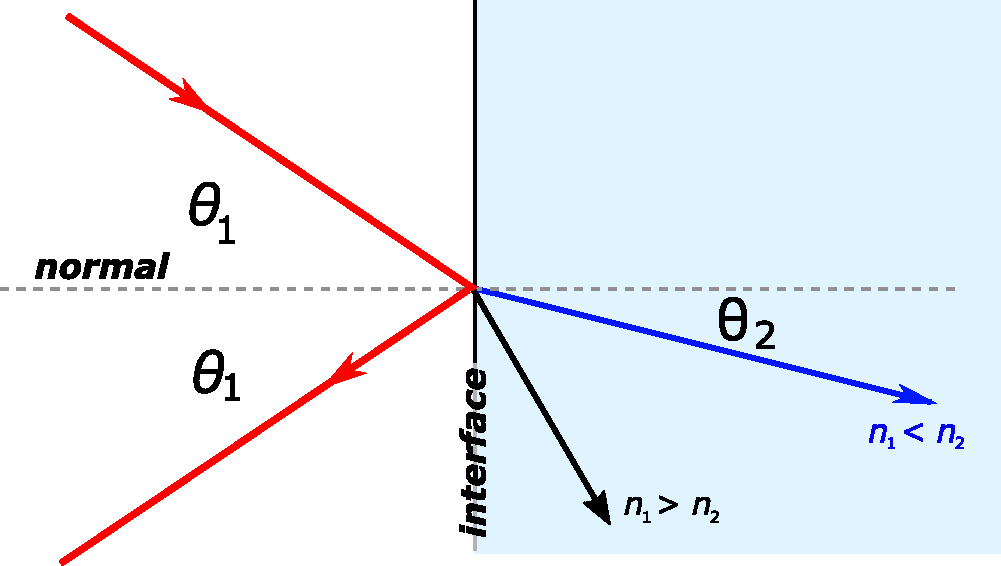
\includegraphics[scale=0.3]{david/index.pdf}
        \caption{Relación entre índice de refracción y el ángulo.}
    \end{figure}
\end{frame}

\section{POLARIZACIÓN}
\subsection{Ondas Linealmente Polarizadas}

\begin{frame}{POLARIZACIÓN}
    \framesubtitle{Ondas Linealmente Polarizadas}
    Cuando una onda tiene desplazamientos sólo en una dirección, se dice que está linealmente polarizada en esa dirección.
    \begin{figure}
        \centering
        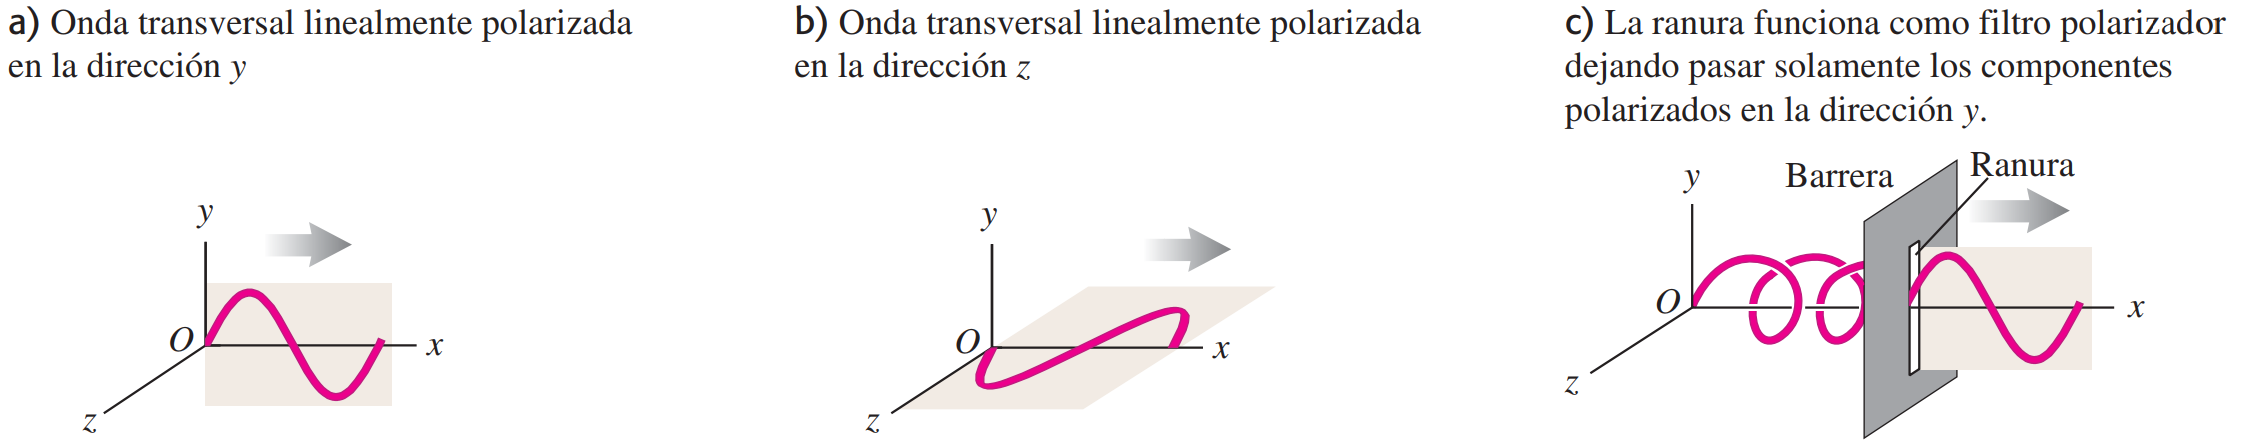
\includegraphics[scale=0.1815]{mari/m_linealpolari.PNG}
        \caption{Ondas linealmente polarizadas\footnotemark{}.}
        \footnotetext{\bibentry{sears}}
    \end{figure}
\end{frame}
%%%%%%%%%%%%%%%%%%%%%%%%%%%%%%%%%%%%%%%
\subsection{Dirección de Polarización}
\begin{frame}{POLARIZACIÓN}
    \framesubtitle{Dirección de Polarización}
    Siempre se define la dirección de polarización de una onda electromagnética como la dirección del vector de campo eléctrico \textbf{E}.
    \begin{equation}
        \overrightarrow{E}(x,t)=\jhat E_{max}\cos\left({kx-\omega t}\right)
    \end{equation}
    \begin{equation}
        \overrightarrow{B}(x,t)=\khat B_{max}\cos\left({kx-\omega t}\right)
    \end{equation}
\end{frame}
%%%%%%%%%%%%%%%%%%%%%%%%%%%%%%%%%%%%%%%%%%
\subsection{Filtros Polarizadores}
\begin{frame}{POLARIZACIÓN}
    \framesubtitle{Filtros Polarizadores}
    El filtro Polaroid incorpora sustancias que presentan dicroísmo, la absorción selectiva en la que una de las componentes polarizadas se absorbe con mucha más intensidad que la otra. Transmite el 80\% o más de la intensidad de una onda que esté polarizada en forma paralela a cierto eje en el material, llamado eje de polarización, pero sólo el 1\% o menos de las ondas polarizadas perpendiculares a ese eje\footnote{\bibentry{sears}.}.

        \begin{figure}
        	\centering
        	\begin{subfigure}[H]{0.4\textwidth}
                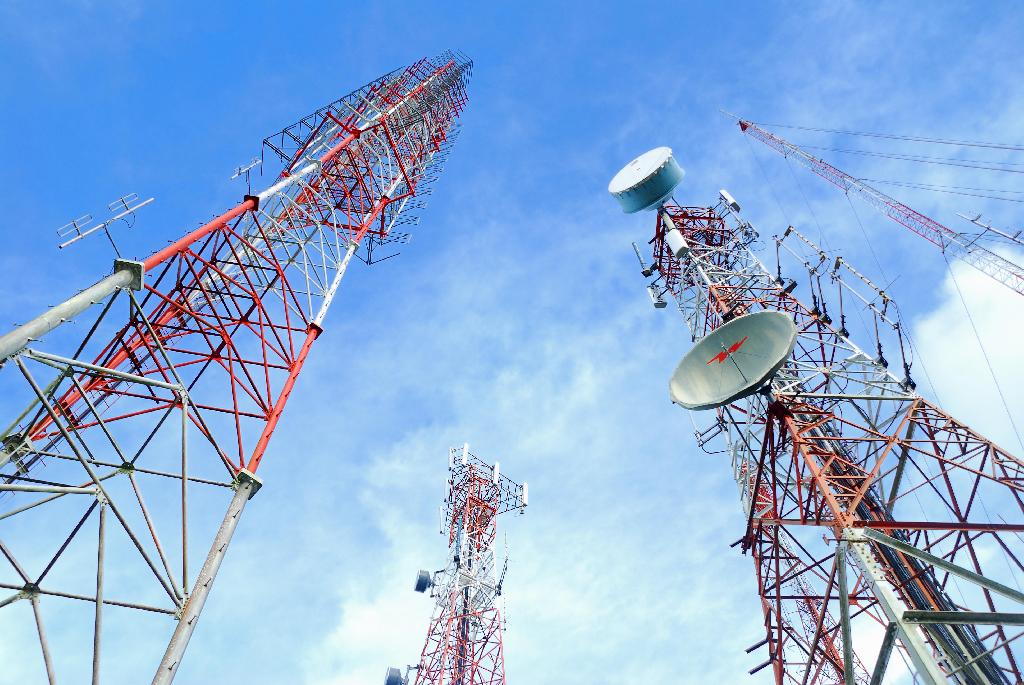
\includegraphics[width=\linewidth]{mari/Antenas.jpg}
                \caption{Antenas telecomunicaciones\footnotemark{}.}
        	\end{subfigure}
            \hspace{2mm}
            \begin{subfigure}[H]{0.32\textwidth}
            	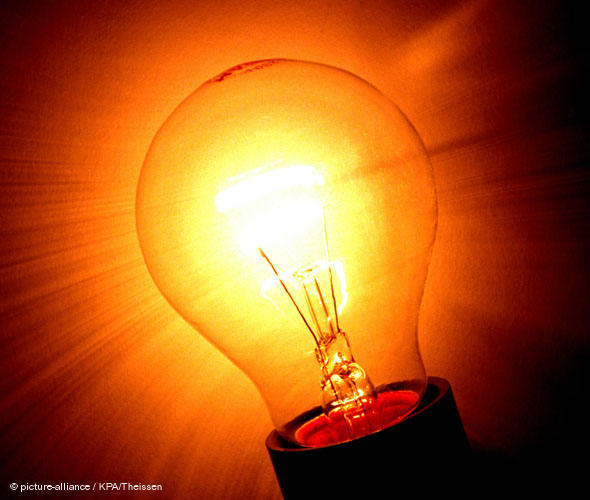
\includegraphics[width=\linewidth]{mari/bombilla.jpg}
                \caption{Bombilla\footnotemark{}.}
            \end{subfigure}
        \end{figure}
        \addtocounter{footnote}{-1}
        \footnotetext{\vspace{-1mm}\bibentry{antena}.}
        \addtocounter{footnote}{1}
        \footnotetext{\bibentry{bombilla}.}
\end{frame}

\begin{frame}{POLARIZACIÓN}
    \framesubtitle{Filtros Polarizadores}
    \begin{figure}[H]
        \centering
        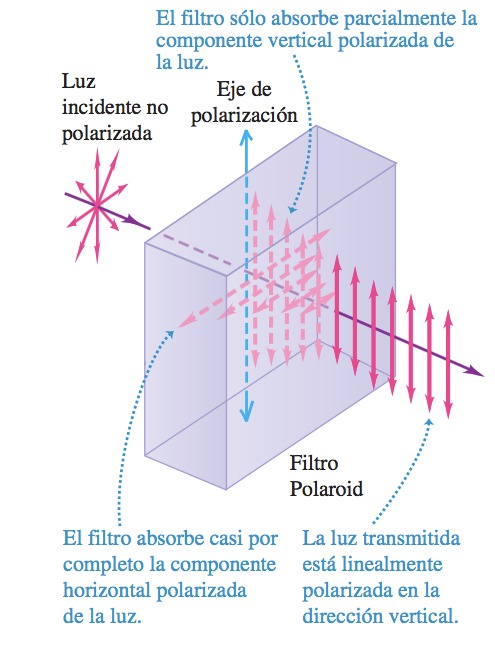
\includegraphics[scale=0.26]{mari/m_filtropolari.jpeg}
        \caption{Filtro polarizador\footnotemark{}.}
    \end{figure}
    \vspace{-10mm}\footnotetext{\bibentry{sears}.}
\end{frame}
%%%%%%%%%%%%%%%%%%%%%%%%%%%%%%%%%%%%%%%%%%%%

\subsection{Ley de Malus}
\begin{frame}{POLARIZACIÓN}
    \framesubtitle{Ley de Malus}
    \begin{figure}[H]
        \centering
        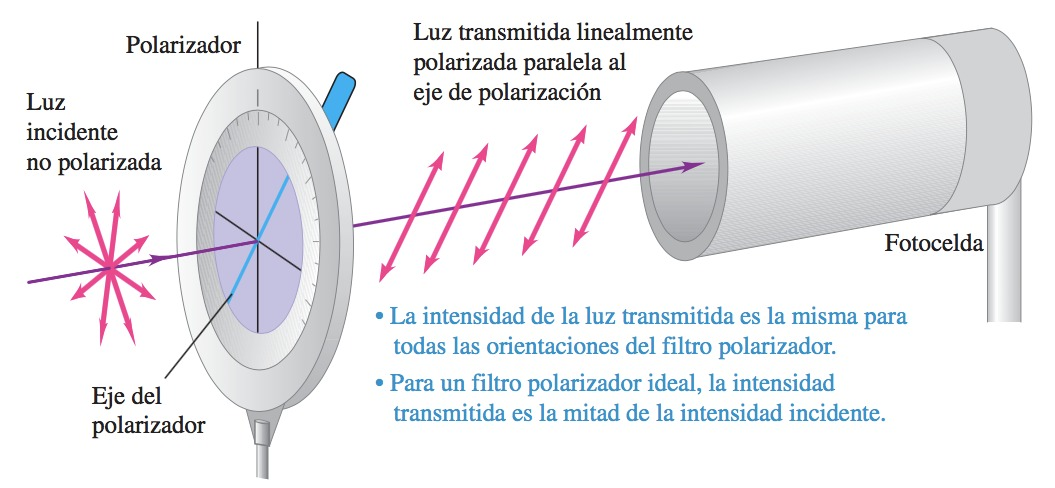
\includegraphics[scale=0.25]{mari/m_malus1.jpeg}
    \end{figure}
    La luz incidente es una mezcla aleatoria de todos los estados de polarización, las componentes paralela y perpendicular al eje de polarización son iguales en promedio, por lo que sólo se transmite la mitad de la intensidad incidente\footnote{\bibentry{sears}}.
\end{frame}

\begin{frame}{POLARIZACIÓN}
    \framesubtitle{Ley de Malus}
    \begin{figure}[H]
        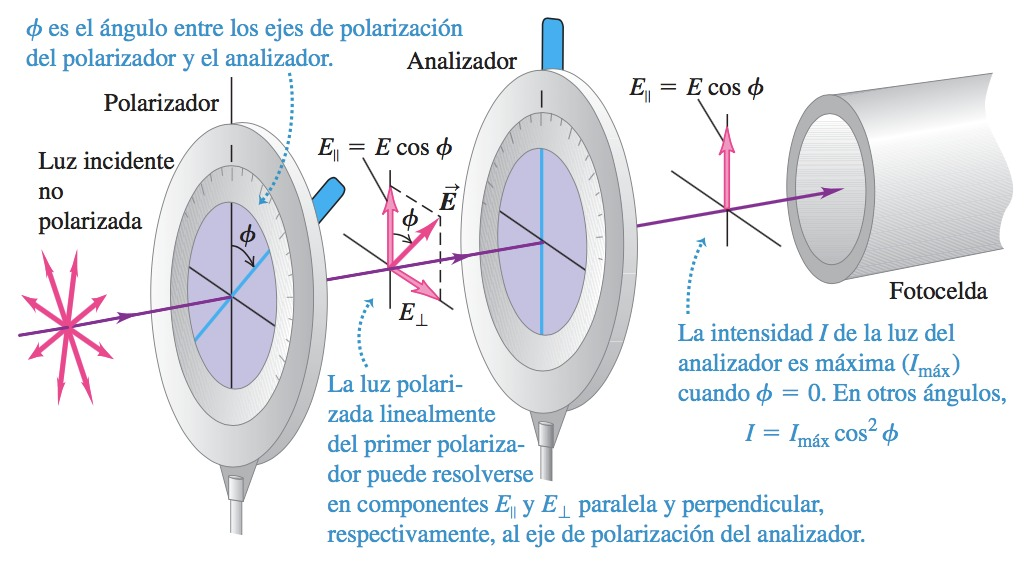
\includegraphics[scale=0.25]{mari/m_malus2.jpeg}
        \caption{Intesidad de luz polarizada\footnotemark{}.}
    \end{figure}
    \footnotetext{\bibentry{sears}}
\end{frame}

\begin{frame}{POLARIZACIÓN}
    \framesubtitle{Ley de Malus}
    Para determinar la intensidad de la luz que sale del analizador debemos saber que la intensidad de una onda electromagnética es proporcional al cuadrado de la amplitud de la onda.
    \begin{equation}
        \begin{split}
            I&=S_{med}=\frac{E_{max}B_{max}}{2\mu_0}=\frac{E_{max}^2}{2\mu_0 c}
            \\&=\frac{1}{2}\sqrt{\frac{\epsilon_0}{\mu_0}}E_{max}^{2}=\frac{1}{2}\epsilon_0 cE_{max}^2
        \end{split}
    \end{equation}

    La razón entre la amplitud trasmitida y la incidente es cos phi, por lo que la razón entre la intensidad transmitida y la incidente es $\cos^2{\phi}$. Así, la intensidad de la luz transmitida a través del analizador es\footnote{\bibentry{sears}}:
    \begin{equation}
        I = I_{max}\cos^2{\phi}
    \end{equation}
\end{frame}
%%%%%%%%%%%%%%%%%%%%%%%%%%%%%%%%%%%%%%%%%%%
\subsection{Polarización por Reflexión}

    %Para cierto ángulo particular de incidencia, llamado el ángulo de polarización, $\theta_p$, la luz cuyo \textbf{E} yace en el plano de incidencia no se refleja en absoluto, sino que se refracta por completo. A ese mismo ángulo de incidencia, la luz cuyo \textbf{E} es perpendicular al plano de incidencia se refleja parcialmente y la otra parte se refracta.
    %\footnotetext{\bibentry{sears}.}


\begin{frame}{POLARIZACIÓN}
    \framesubtitle{Polarización por Reflexión}
    En 1812 el científico británico Sir David Brewster descubrió que cuando el ángulo de incidencia es igual al ángulo de polarización $\theta_p$, el rayo reflejado y el rayo refractado son perpendiculares entre sí.
    \begin{equation}
        \tan{\theta_p}=\frac{n_b}{n_a}
    \end{equation}
    \begin{figure}
        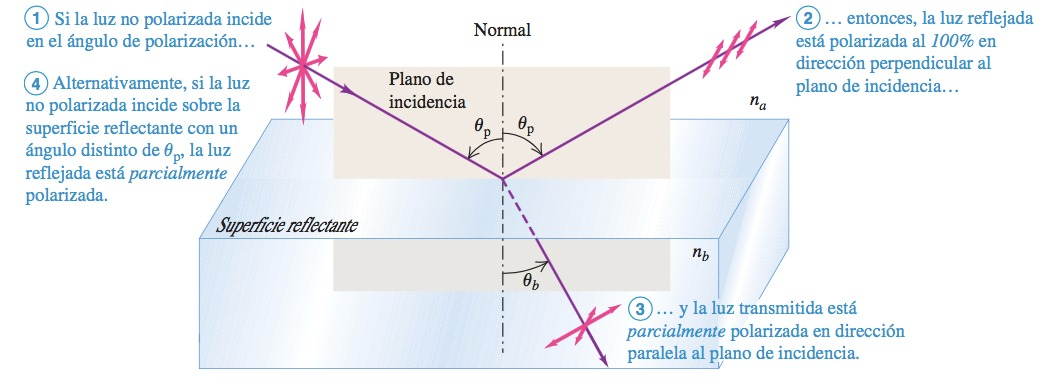
\includegraphics[scale=0.2775]{mari/m_reflex.jpeg}
        \caption{Ley de Brewster para el ángulo de polarización\footnotemark{}.}
    \end{figure}
    \vspace{-1cm}\footnotetext{\bibentry{sears}.}
\end{frame}

\section{INTERFEROMETRÍA}

\subsection{Introducción}
\begin{frame}{INTERFEROMETRÍA}
	\framesubtitle{Introducción}

	¿Qué ocurre cuando dos ondas del mismo tipo se encuentran?

	\url{https://www.youtube.com/watch?v=1PuzdU2RvW8}
	\url{https://www.youtube.com/watch?v=faAPLf7yPkl}

	%%%Imagen: http://www.principiamarsupia.com/wp-content/uploads/2016/02/pond.jpg
\end{frame}



\subsection{Interferencia Constructiva y Destructiva}

\begin{frame}{INTERFEROMETRÍA}
	\framesubtitle{Interferencia Constructiva y Destructiva}
	Para interferencia constructiva:
	\begin{equation}
		\Delta x = m \lambda , m=0, \pm 1, \pm 2...
	\end{equation}
	Para interferencia destructiva:
	\begin{equation}
		\Delta x = \frac{m\lambda}{2} , m=1, 3, 5...
	\end{equation}

  \begin{figure}
    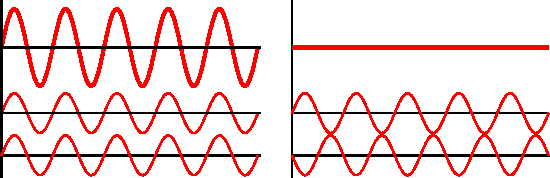
\includegraphics[scale=1]{juanse/interference.pdf}
    \caption{Interferencia entre ondas\footnotemark{}.}
  \end{figure}
  \vspace{-5mm}\footnotetext{\bibentry{interferencia}}
\end{frame}



\subsection{Inteferómetro de Michelson}
\begin{frame}{INTERFEROMETRÍA}
	\framesubtitle{Interferómetro de Michelson}
  \begin{figure}
    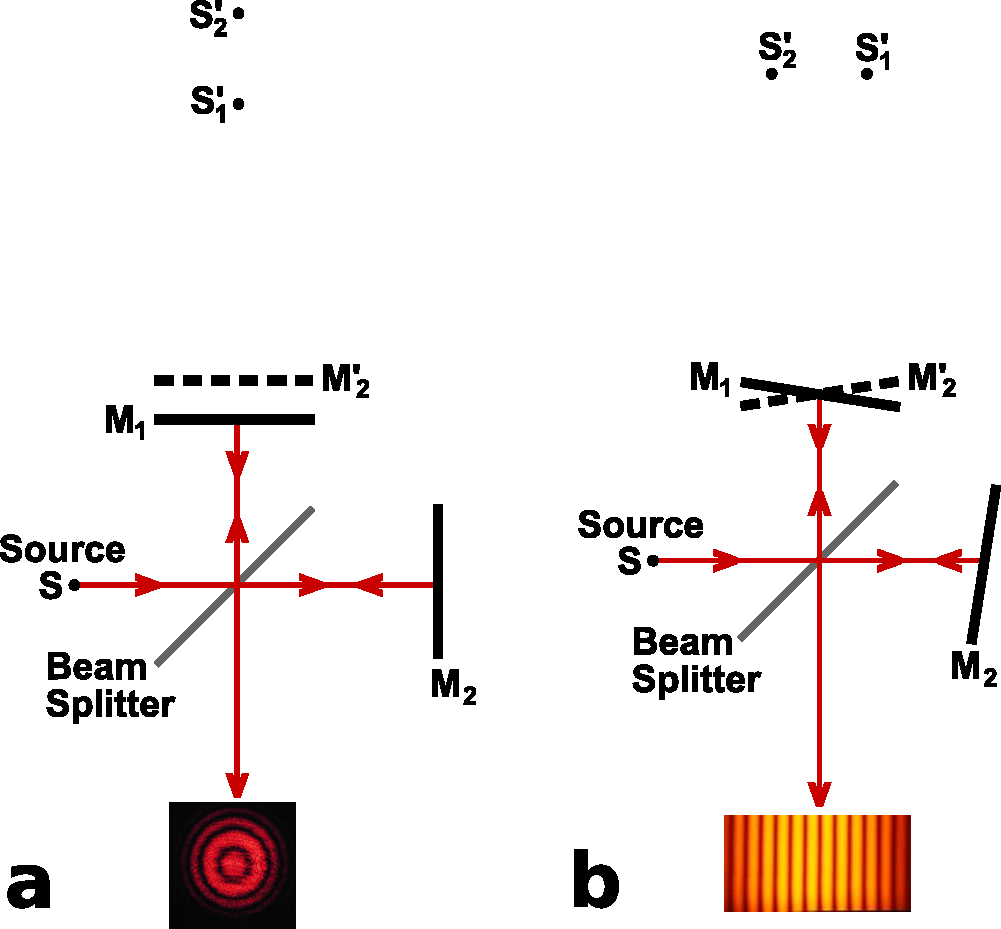
\includegraphics[scale=0.34]{juanse/michelson.pdf}
    \caption{Interferómetro de Michelson\footnotemark{}.}
  \end{figure}
  \vspace{-5mm}\footnotetext{\bibentry{michelson}}
\end{frame}




\subsection{Aplicaciones}

\begin{frame}{INTERFEROMETRÍA}
\framesubtitle{Aplicaciones}
\begin{multicols}{2}
	\textbf{Medición de Ondas Gravitacionales\\}
	Este interferómetro, en conjunto con cavidades de Fabry-Perot, permitió a LIGO medir la existencia de ondas gravitacionales
	en el 2015\footnote{\bibentry{ligo}}.
	\vfill\null

	\textbf{Experimento de Michelson-Morley\\}
	En 1920, Michelson y Morley intentaron demostrar la existencia del éter por medio de esta configuración. Sin embargo, no se logró demostrar su existencia.
\end{multicols}
\url{https://ligo.caltech.edu/system/video_items/files/21/Einsteins_messengers_hi_res_Nov_17_MPEG720p.mp4?1447873693}
\end{frame}

\begin{frame}{INTERFEROMETRÍA}
	\framesubtitle{Aplicaciones}
	\begin{multicols}{2}

	\textbf{Medir calidad de una superficie\\}

	La interferometría se puede utilizar para medir qué tan plana es una superficie, por medio de las franjas que éste presenta.

	\vfill\null

	\textbf{Interferómetro de Twyman-Green\\}
	Es una variación del interferómetro de Michelson para probar el funcionamiento de algun tipo de lente.
\end{multicols}
	\begin{figure}
		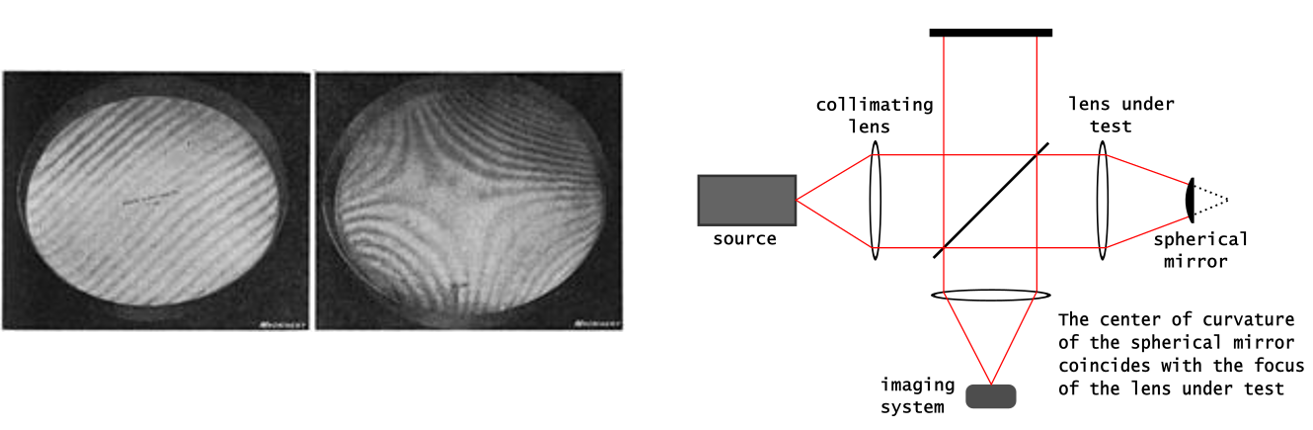
\includegraphics[scale=0.4]{juanse/twyy.png}
		\caption{Algunas aplicaciones de la interferometría\footnotemark{}\footnotemark{}.}
	\end{figure}
	\addtocounter{footnote}{-1}
	\footnotetext{\bibentry{fringes}}
	\addtocounter{footnote}{1}
	\footnotetext{\bibentry{twy}}
	\vspace{-1cm}
\end{frame}


\section{DIFRACCIÓN}
\subsection{Concepto}

\begin{frame}{DIFRACCIÓN}
    \framesubtitle{Concepto}
    Un objeto opaco que se interpone entre una fuente de luz y una superficie, una pared por ejemplo, la sombre que se observa no es totalmente nítida\footnote{\bibentry{sears}}.
    \begin{figure}[H]
		\centering
		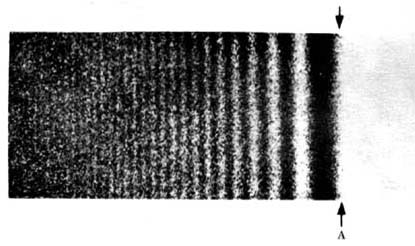
\includegraphics[scale=1]{david/Shadow.jpg}
		\caption{Acercamiento al borde de una sombra \footnotemark{}.}
	\end{figure}
    \footnotetext{\bibentry{Shadow}}
    \begin{itemize}
        \item Fallan las predicciones de la óptica geométrica.
        \item Franjas brillantes y oscuras alternadas.
    \end{itemize}
    \vspace{-5mm}
\end{frame}

\begin{frame}{DIFRACCIÓN}
    \framesubtitle{Concepto}
    También se puede definir como los patrones de interferencia que se forman cuando la luz incide en una barrera que cuenta con una abertura o un borde. Pero, en general, aplica para todo tipo de ondas \footnote{\bibentry{sears}}.
    \begin{figure}[H]
		\centering
		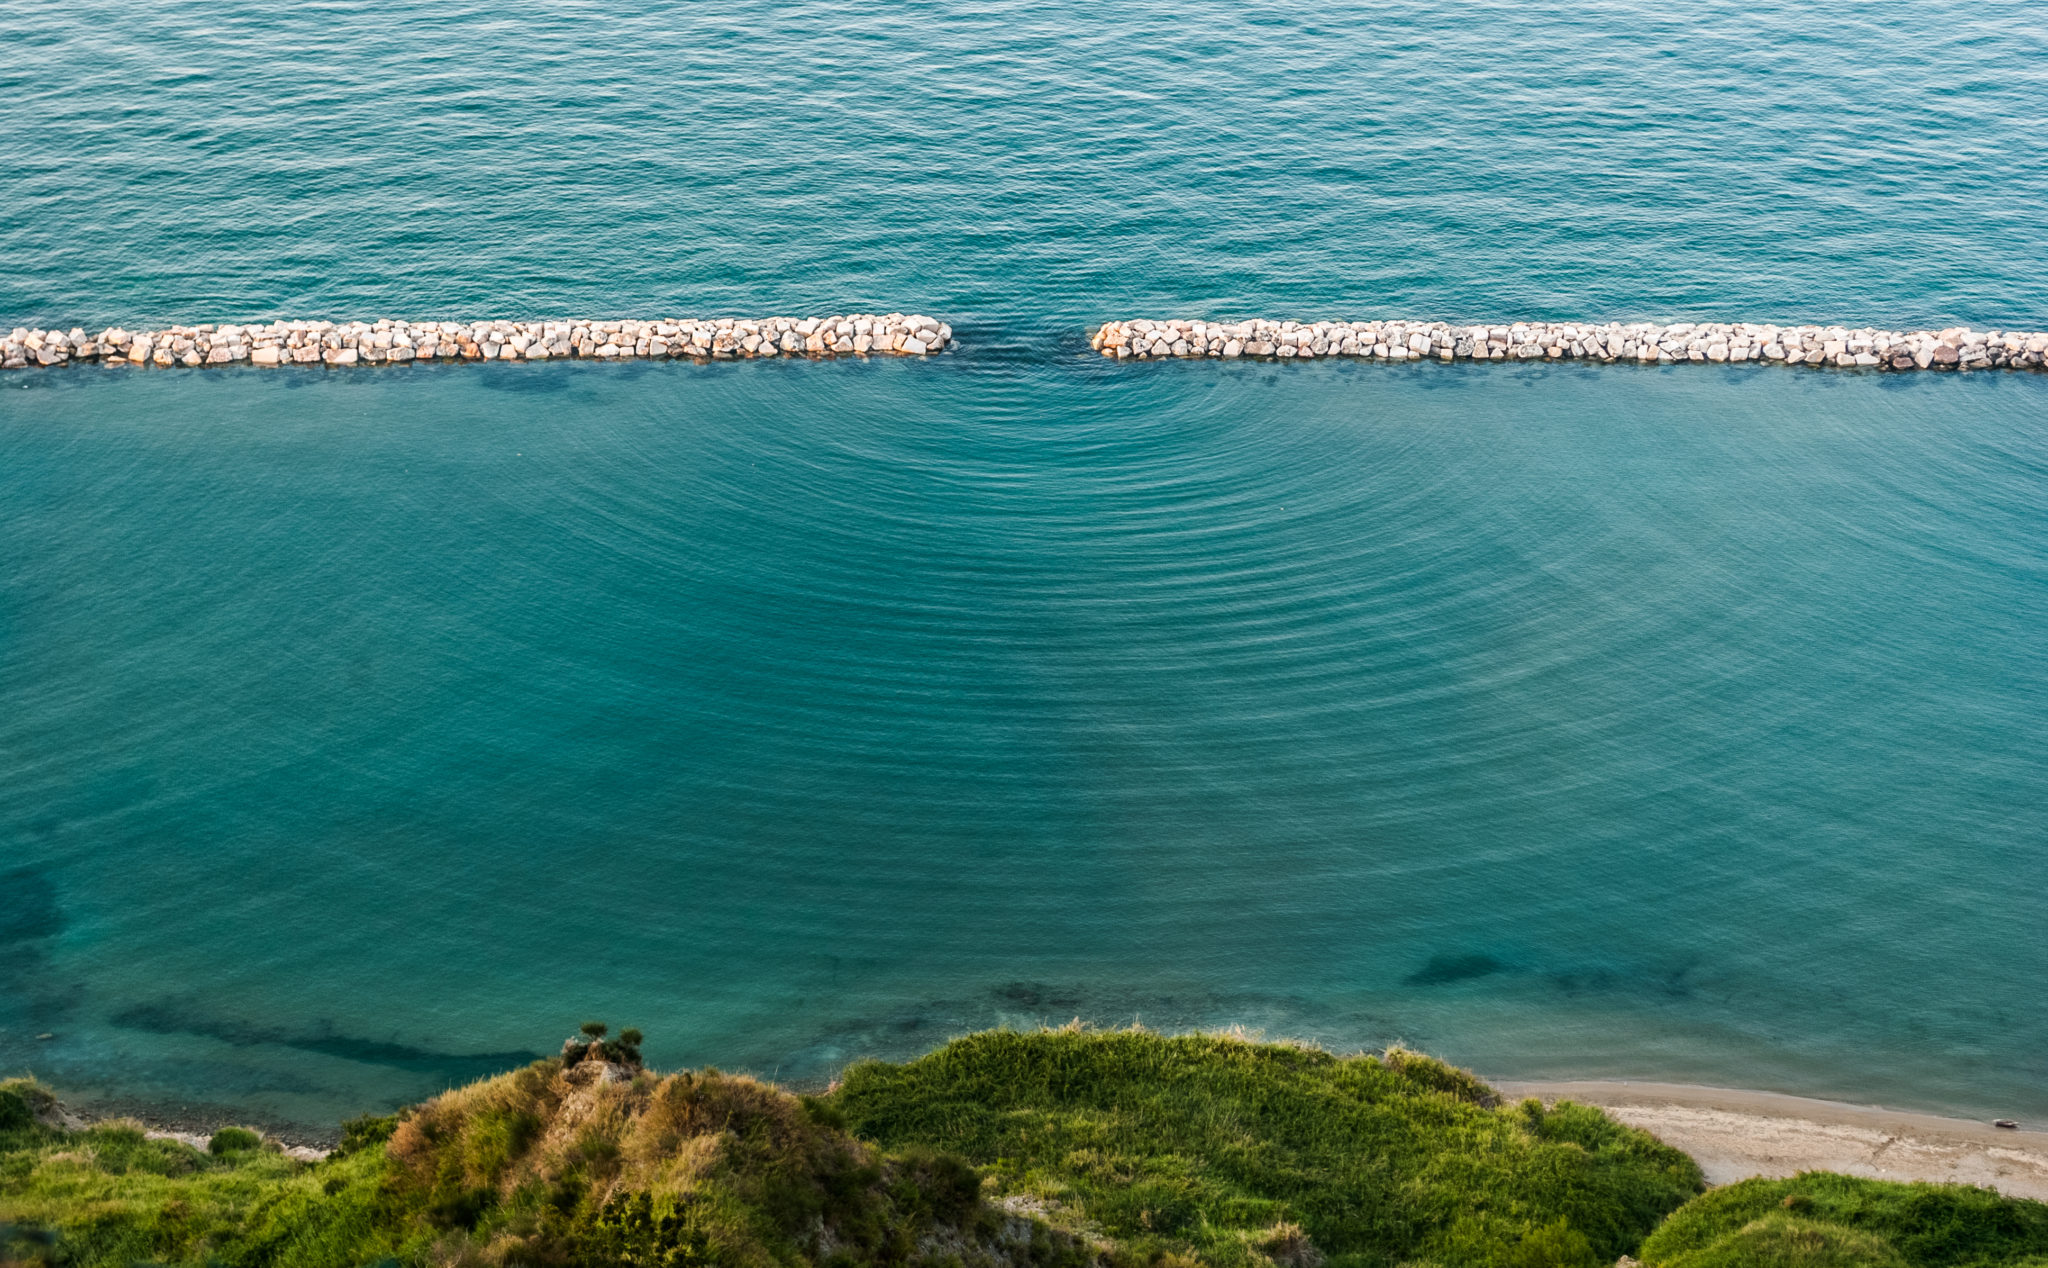
\includegraphics[scale=0.35]{david/waterwave.jpg}
		\caption{Difracción de una onda en el mar\footnotemark{}.}
	\end{figure}
    \vspace{-1cm}\footnotetext{\bibentry{waterwave}}
\end{frame}

\begin{frame}{DIFRACCIÓN}
    \framesubtitle{Principio de Fresnel-Huygens}
    \textit{"Todo punto de un frente de onda inicial puede considerarse como una fuente de ondas esféricas secundarias que se extienden en todas las direcciones con la misma velocidad, frecuencia y longitud de onda que el frente de onda del que proceden" \footnote{\bibentry{hecht}}}.
    \begin{figure}
        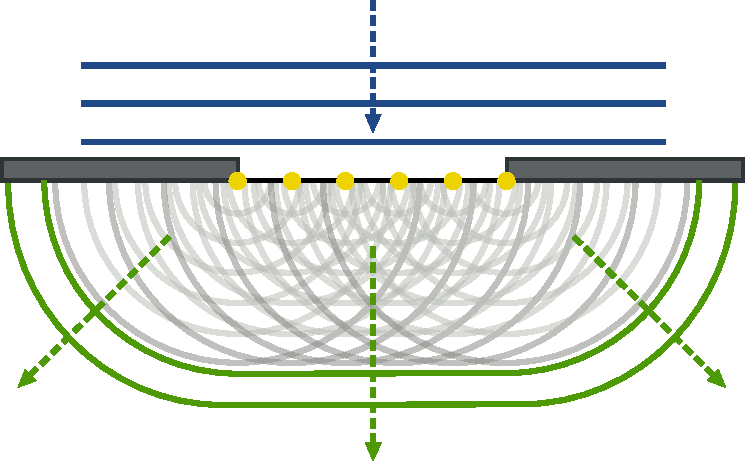
\includegraphics[scale=0.53]{david/huygens.pdf}
        \caption{Principio de Huygens a través de una rendija.}
    \end{figure}
\end{frame}

\subsection{Patrón de Difracción}
\begin{frame}{DIFRACCIÓN}
    \framesubtitle{Patrón de Difracción}
    Imagen de la modulación de la intensidad de la onda debido a la difracción.  El patrón de difracción se construye a partir de la superposicion de todas las ondas que plantea Fresnel-Huygens\footnote{\bibentry{hecht}}.
    \begin{figure}
        \centering
        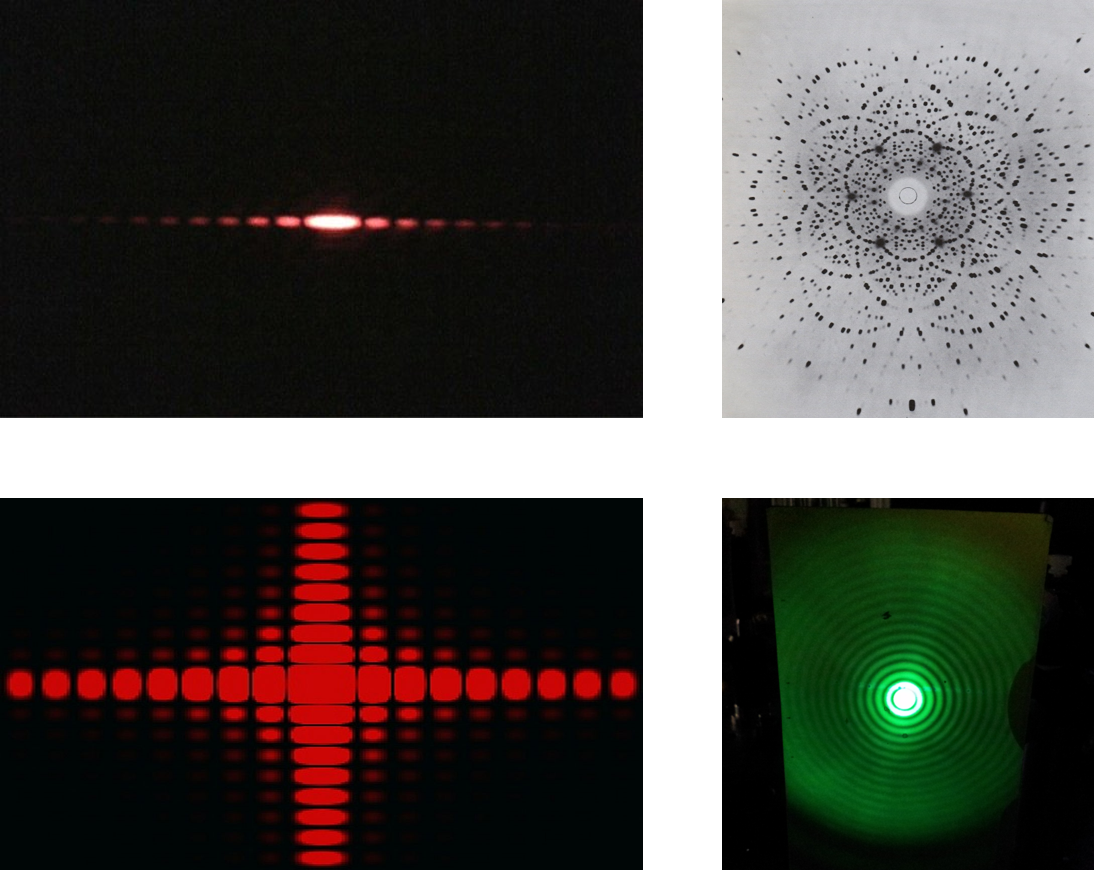
\includegraphics[scale=0.295]{david/Diff.png}
        \caption{Diferentes patrones de difracción.}
    \end{figure}
    \vspace{-2cm}
\end{frame}

\subsection{Enfoques}
\begin{frame}{DIFRACCIÓN}
    \framesubtitle{Enfoques}
    \begin{multicols}{2}
        \textbf{Fresnel}\\
            Se considera la curvatura de las ondas salientes de la abertura de difracción. Normalmente ocurre cuando la abertura está muy cerca a la pantalla de observación.
        \vfill\null
        \textbf{Fraunhofer}\\
            Se considera difracción de Fraunhofer cuando las ondas salientes de la rendija con casi planas comparadas con la fuente\footnote{\bibentry{hecht}}.
    \end{multicols}
    \begin{figure}[H]
        \centering
        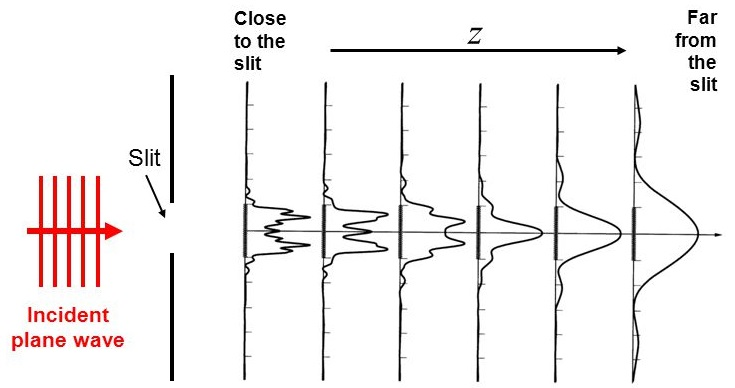
\includegraphics[scale=0.3]{david/enfoques.jpg}
        \caption{Intensidad de acuerdo al enfoque de estudio\footnotemark{}.}
    \end{figure}
    \footnotetext{\bibentry{Wilcox}}
    \vspace{-1.5cm}
\end{frame}

\begin{frame}{DIFRACCIÓN}
    \framesubtitle{¿Qué tanto se difracta una onda?}
    La difracción depende de qué tan comparable sea un obstáculo con la longitud de onda.
    \begin{figure}
        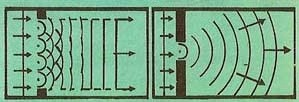
\includegraphics[scale=0.5]{david/wavelength.jpg}
        \caption{Comparación de una onda incidente respecto a rendijas.}
    \end{figure}

    \begin{figure}
        \centering
        \begin{subfigure}[H]{0.25\textwidth}
            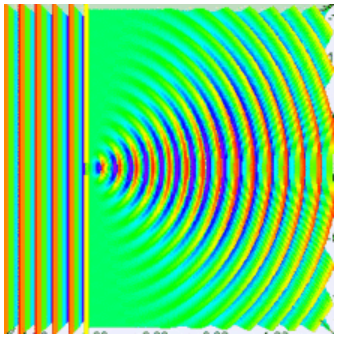
\includegraphics[width=\linewidth]{david/narrow.PNG}
        \end{subfigure}
        \hspace{2mm}
        \begin{subfigure}[H]{0.25\textwidth}
            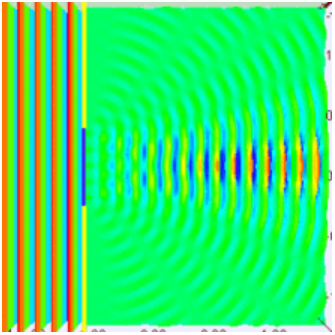
\includegraphics[width=\linewidth]{david/wide.PNG}
        \end{subfigure}
        \caption{Propagación de acuerdo a las rendijas\footnotemark{}.}
    \end{figure}
    \vspace{-1cm}\footnotetext{\bibentry{wikiwave}}

\end{frame}

\subsection{Experimento de una Rendija}
\begin{frame}{DIFRACCIÓN}
    \framesubtitle{Experimento de una Rendija}
    Hay una onda incidente en la abertura, la abertura se considera como una fuente continua de ondas esféricas\footnote{\bibentry{sears}}.
    \begin{equation}
        I=I_0\left\{\frac{\sin\left[\pi a \left(\sin\theta\right)/\lambda\right]}{\pi a\left(\sin\theta\right)/\lambda}\right\}^2
    \end{equation}
    \vspace{-5mm}
    \begin{figure}
        \centering
        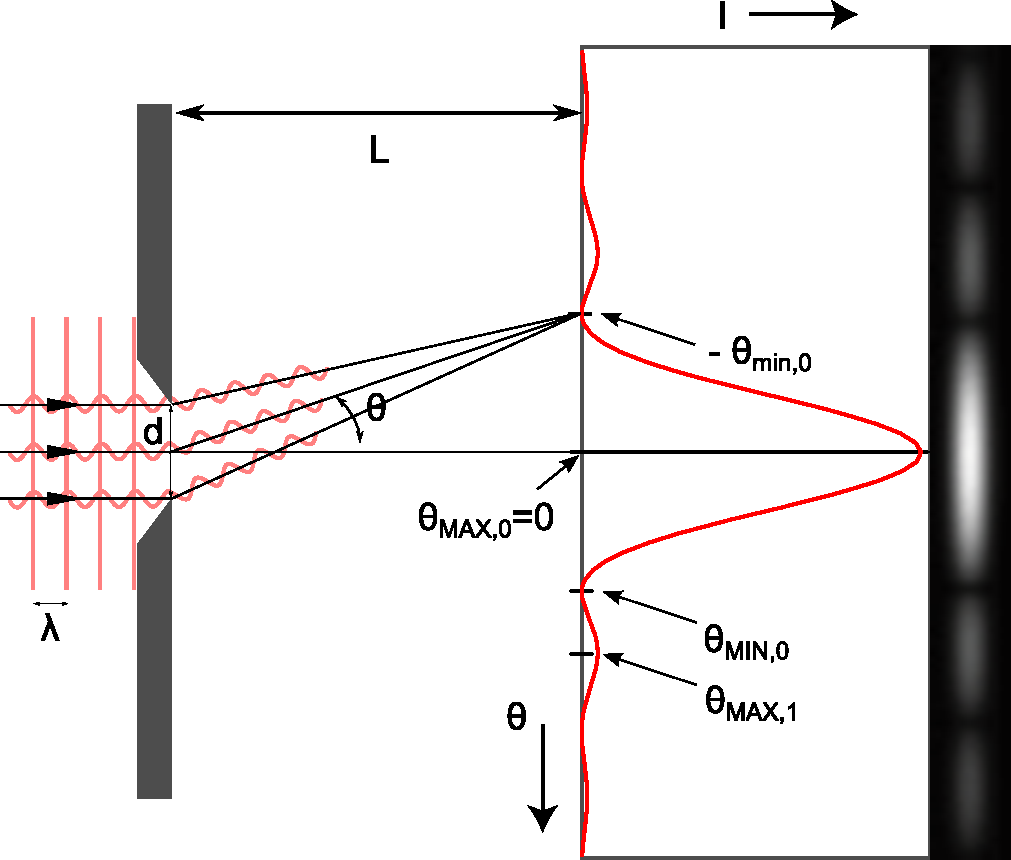
\includegraphics[scale=0.25]{david/singleSlit.pdf}
        \caption{Difracción, intensidad y patrón de difracción para una rendija.}
    \end{figure}
    \vspace{-2cm}
\end{frame}

\subsection{Experimento de Young}

\begin{frame}{DIFRACCIÓN}
    \framesubtitle{Experimento de Young}
    \textbf{¿Qué esperaríamos ver?\\}
	Si la luz se comportara como una partícula, se esperaría observar:
	 \begin{figure}
         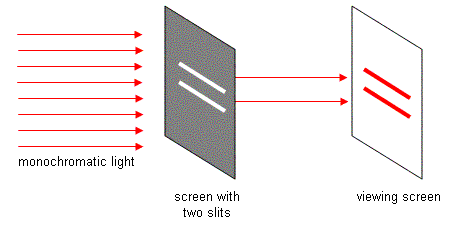
\includegraphics[scale=0.7]{juanse/young_particle.png}
         \caption{Resultado esperado del modelo como partícula\footnotemark{}.}
     \end{figure}
     \footnotetext{\bibentry{young1}}
\end{frame}

\begin{frame}{DIFRACCIÓN}
    \framesubtitle{Experimento de Young}
    \begin{figure}
        \centering
        \begin{subfigure}[H]{0.4\textwidth}
            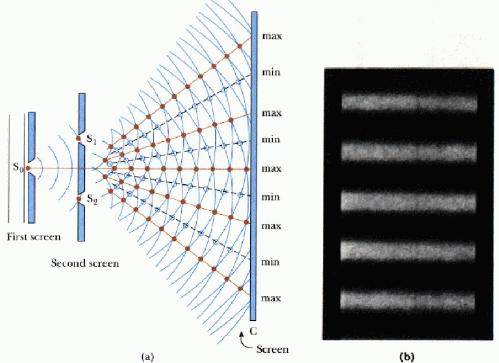
\includegraphics[width=\linewidth]{juanse/waves.png}
            \caption{Patrón de Interferencia\footnotemark{}.}
        \end{subfigure}
        \hspace{2cm}
        \begin{subfigure}[H]{0.4\textwidth}
            \only<1>{}
            \only<2>{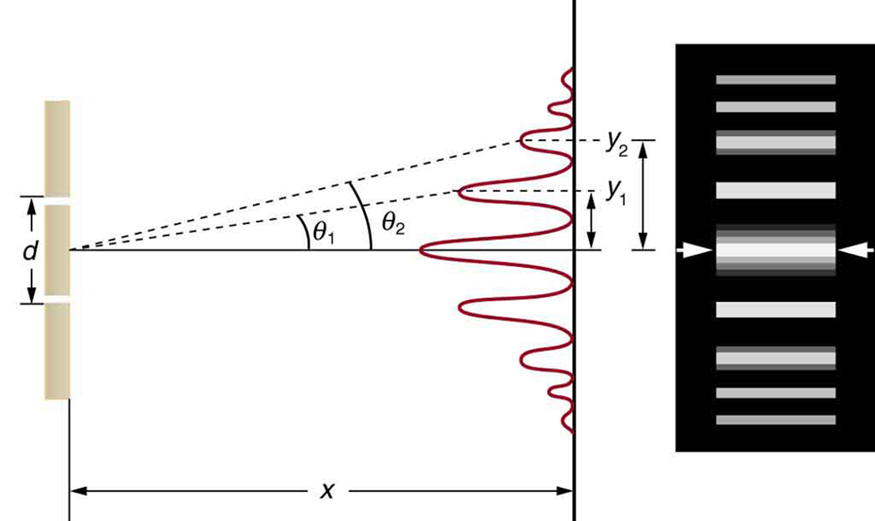
\includegraphics[width=\linewidth]{juanse/waves2.jpg}
            \caption{Patrón de Intensidad\footnotemark{}.}}
        \end{subfigure}
    \end{figure}
    \addtocounter{footnote}{-1}
    \footnotetext{\bibentry{youngwaves}}
    \addtocounter{footnote}{1}
    \footnotetext{\bibentry{youngwaves2}}
\end{frame}


\subsection{Difracción de Rayos X}
\begin{frame}{DIFRACCIÓN}
    \framesubtitle{Rayos X}
    Los rayos X fueron descubiertos por Wilhelm Röntgen en 1895; tienen longitudes del orden de $10^{-10}\,m$. Pueden utilizarse para determinar defectos en componentes técnicos, como tuberías, turbinas, motores, paredes, vigas, y en general casi cualquier elemento estructural\footnote{\bibentry{sears}}.
    \begin{figure}
        \centering
        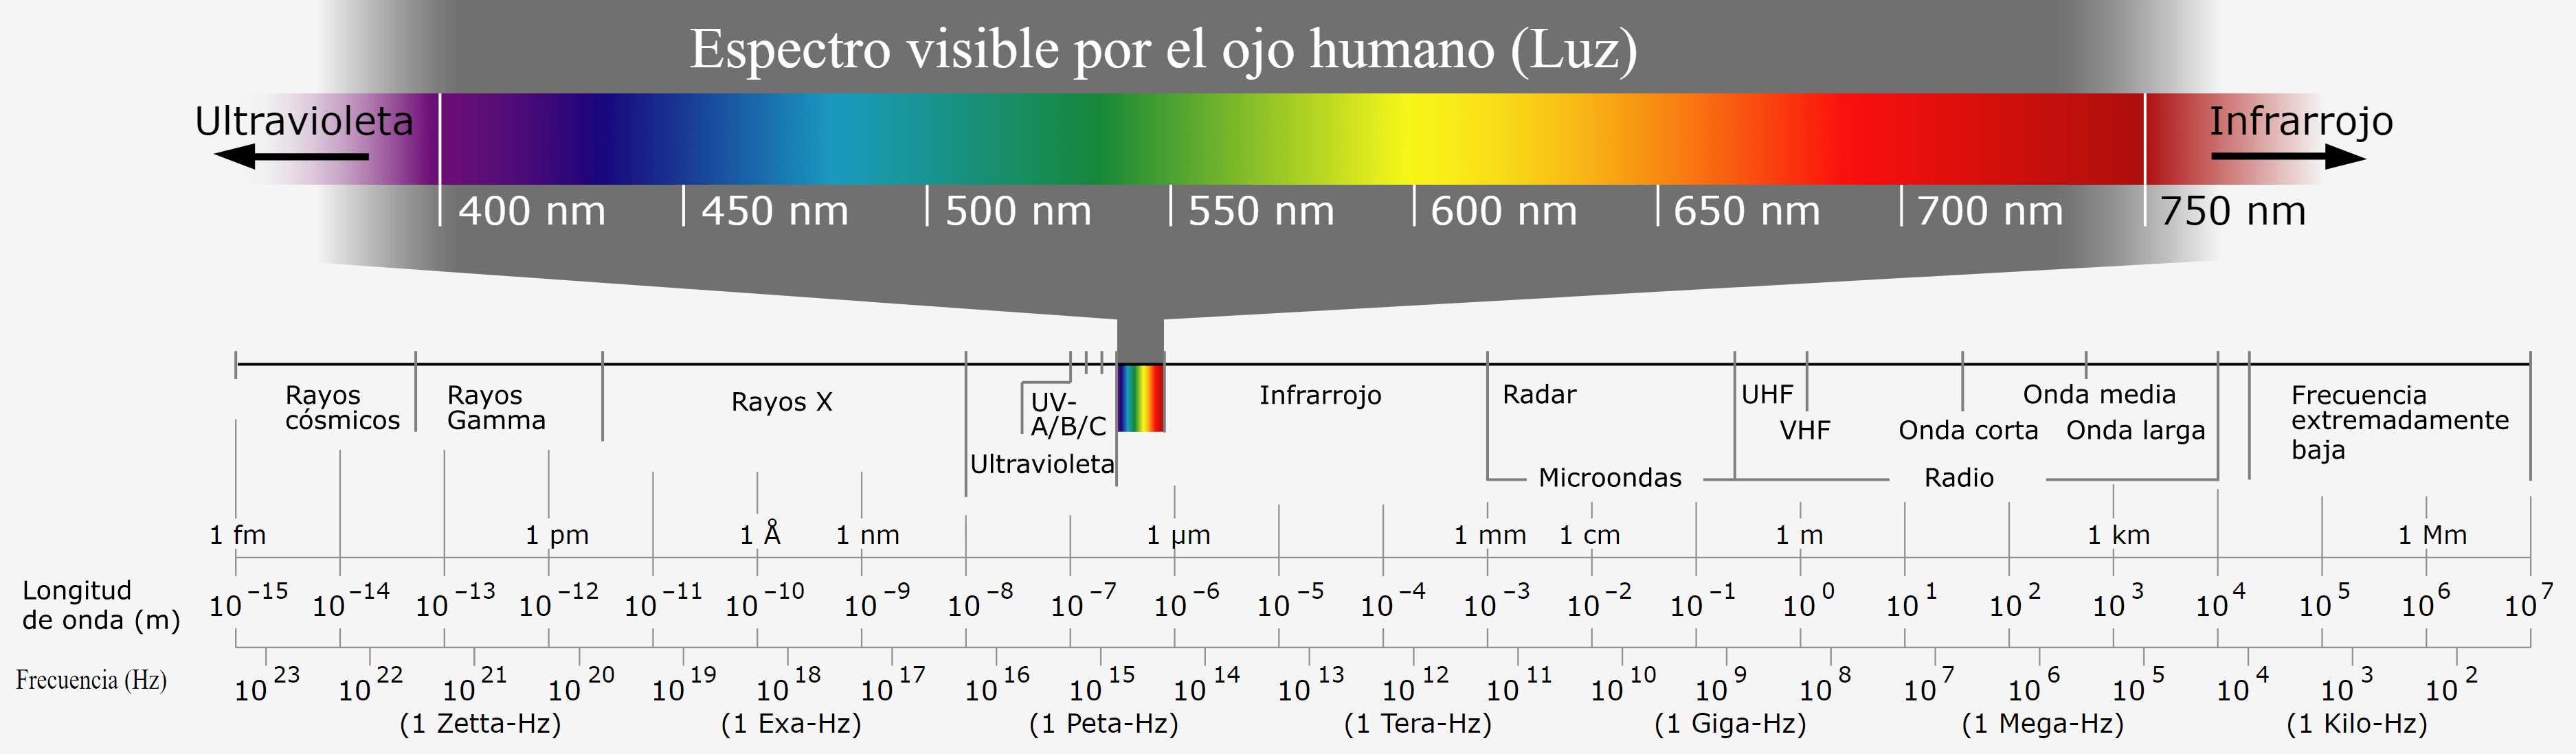
\includegraphics[scale=0.084]{david/espectro.png}
        \caption{Espectro electromagnético\footnotemark{}.}
    \end{figure}
    \vspace{-5mm}\footnotetext{\bibentry{espectro}}
\end{frame}



\begin{frame}{DIFRACCIÓN}
    \framesubtitle{Difracción de Rayos X}
    En 1912, Max von Laue propuso la idea de que un cristal podría servir como una rejilla de difraccion tridimensional para los rayos X.
    \begin{figure}[H]
		\centering
		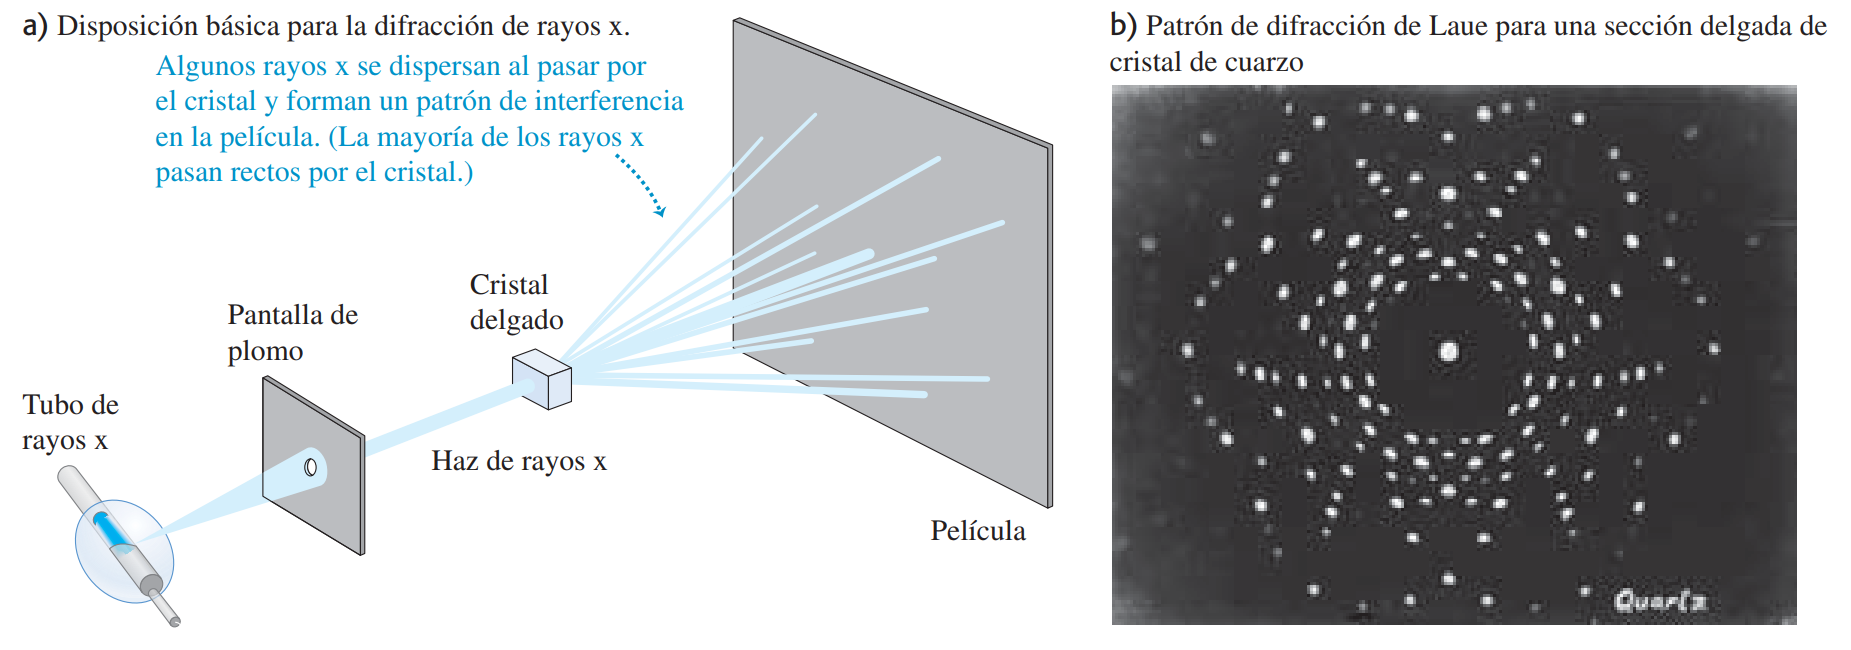
\includegraphics[scale=0.1975]{david/Laue.PNG}
		\caption{Experimento de Laue \footnotemark{}.}
	\end{figure}
    \footnotetext{\bibentry{sears}}
    Resultó en la prueba experimental de que los rayos X son, en efecto, una onda electromagnética.
    \vspace{-1cm}
\end{frame}

\begin{frame}{DIFRACCIÓN}
    \framesubtitle{Difracción de Rayos X}

\end{frame}

\nonumb % Not numbered titles
%\addcontentsline{toc}{section}{\small\protect\numberline{}{REFERENCIAS BIBLIOGRÁFICAS}} % Separated from other contents, for small number of contents
\addcontentsline{toc}{section}{\small REFERENCES} % Closer from other contents, for large number of contents
\nocite{*} % All citations showed (take care with fraud!)
%%%%%%%%%%%%%%%%%%%%%%%%%%%%%%%%%%%%%%%%%%%%%%%%%%%%%%%%%%%%%%%%%%%%%%%%%%%%
\section*{REFERENCES}
\begin{frame}[allowframebreaks]{REFERENCES} %  and put before {REFEREN...}
\begingroup % Group for changing the color
\renewcommand{\color}[1]{} % Allows to have black bibs and white footnote bibs
\small{\bibliographystyle{IEEEtran}} % Size of text; acm or gatech-thesis or ieeetr or ieeetran or icontec or iso690
\bibliography{ref}
\endgroup % Group for changing the color
% pdflatex -> bibtex -> pdflatex -> pdflatex
\end{frame}
%%%%%%%%%%%%%%%%%%%%%%%%%%%%%%%%%%%%%%%%%%%%%%%%%%%%%%%%%%%%%%%%%%%%%%%%%%%%
% Thank-slide
\begin{frame}[plain,noframenumbering] % No frame number
	\begin{beamercolorbox}[ht=\paperheight,wd=\paperwidth, center]{Portada}
		\begin{center}\Huge\textbf{Thank you}\end{center} % Or Thanks; leave the next space mandatorily
		
		\vspace{0.44\paperheight}
    \end{beamercolorbox}
\end{frame}
%%%%%%%%%%%%%%%%%%%%%%%%%%%%%%%%%%%%%%%%%%%%%%%%%%%%%%%%%%%%%%%%%%%%%%%%%%%%



\end{document}
